\documentclass[11pt]{article}
\usepackage{listings}
\usepackage{graphicx}

\title{\textbf{Project 2 - Failure Model\\ COP5615}}
\author{Rahul Prabhu\\
		Sanil Sinai Borkar}
\date{\today}

\usepackage[parfill]{parskip}
\begin{document}

\maketitle

\section{Description}
The program was run with an additional parameter which indicated the percentage of the network that needs to go down. The following command was run at the command prompt:
\begin{lstlisting}
$ run <num_of_nodes> <topology> <algorithm> <percent_failure>
\end{lstlisting}


There are 4 command-line arguments as given below:
\begin{enumerate}
\item \textbf{num\_of\_nodes}: The number of nodes in the network topology. It is a positive integer value.
\item \textbf{topology}: The network topology. It should be one of `full', `line', `3D' or `imp3D'.
\item \textbf{algorithm}: The algorithm. It should be either `gossip' (Gossip Protocol) or `push-sum' (Push-Sum Algorithm).
\item \textbf{percent\_failure}: Percent of the total number of nodes that need to fail.
\end{enumerate}

If the number of nodes that need to fail is a real number, it was `floored' to the nearest integer.

We tested the performance in case of both temporary and permanent failures. Temporary failure was achieved by sending a message to the designated actor asking forcing it to go to sleep for a specific amount of time. Permanent failure was achieved by maintaining the current `state' of an actor. It was initialized to the ``ALIVE" state, and was switched to ``DEAD" state to simulate its death. Once ``DEAD", it never came back up.

\section{Gossip Protocol}
The Gossip Protocol took a lot more time to converge than the normal implementation. Figure~\ref{gossip_failure} shows the percentage coverage a network reached on different failure rates and different topologies.

\textit{For each combination of parameters, we ran the program a few times. The average of all the runs was then considered for our analyses and the graph plots.}
\begin{figure}[h]
    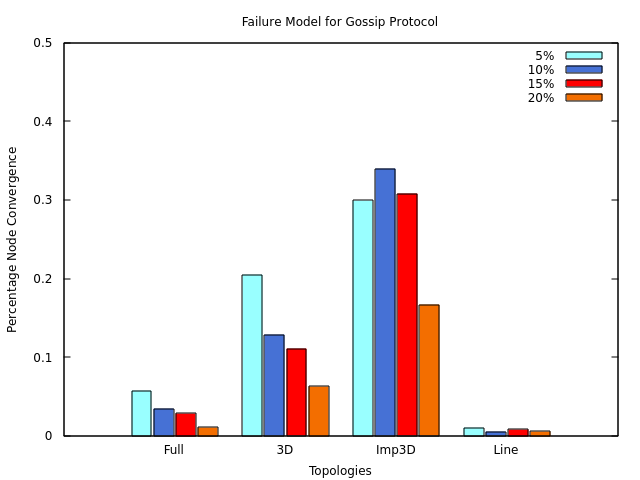
\includegraphics[scale=0.75]{gossip_failure.png}
    \caption{Gossip Protocol Run on various topologies with different percentage of nodes failing.}
    \label{gossip_failure}
\end{figure}

\section{Push-Sum Algorithm}
As expected, the Push-Sum took a lot more time to converge to the correct average value than the normal implementation. Figure~\ref{pushsum_failure} shows the time taken for convergence on different failure rates and different topologies.
\begin{figure}[h]
    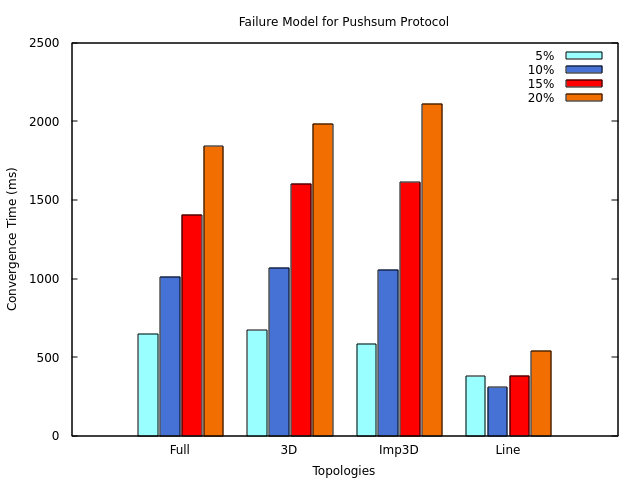
\includegraphics[scale=0.75]{pushsum_failure.png}
    \caption{Push Sum Protocol Run on various topologies with different percentage of nodes failing.}
    \label{pushsum_failure}
\end{figure}

\textit{For each combination of parameters, we ran the program a few times. The average of all the runs was then considered for our analyses and the graph plots.}

\section{Observations}
In case of temporary failures, once the node was up and running, the protocol continued running and eventually converged. However, this process took a longer time.

In case of permanent failures, the protocol execution was stopped. Since the node failed, there was a portion of the network that was disconnected. As a result, convergence was not achieved.

The time does not monotonically decrease as we increase the number of failure nodes as it actually depends on which nodes fail. This is evident from the graph plots of the Gossip Protocol for permanent nodes failures, particularly in case of line and imperfect 3D topologies.

Out of all the topologies that we worked with, the line topology is the most inflexible, prone to disconnection, and most unpredictable topologies. Since a node can send a message only to 2 of its neighbors (left and right), if one of these nodes go down, it takes a very long time for the algorithm to converge. Also, the output for the same number of nodes is highly inconsistent.

\end{document}
